% !TeX root = report.tex
% !TeX encoding = UTF-8
% !TeX spellcheck = en_US
%
% Report for Train a Smartcab to Drive
% Udacity MLND Project 4
%
% Aravind Battaje

\documentclass{article}

% Packages used
\usepackage[margin=1in]{geometry}
\usepackage{amsmath}
\usepackage{graphicx}
\usepackage{caption}
\usepackage{hyperref}

% Begin document
\begin{document}
	
	\title{Project Report: Train a Smartcab to Drive}
	\author{Aravind Battaje}
	\maketitle
	
	\section{Project steps}	
	The task is to use reinforcement learning techniques to train a ``smartcab'' to find an optimal path between source and destination in an idealized city setting. A learning agent is implemented in a simulation environment already provided with the project. The learning agent learns to use actions in the environment which are generally rewarded for such as following traffic rules and reaching destination. The agent starts with no knowledge of its environment, apart from the potential number of states that the actor (agent) can reach, and gradually learns by using a exploration heavy approach initially, followed by finding the actions that lead to maximum rewards. Every action taken at an instant is supplied to a Q-Learning method that models the utilities of several states, given an action. The Q-Learner is allowed to learn over multiple trials (source to destination within some time), with successive trials characterizing more confident understanding of the world. Given some reasonable parameters, the agent learns to reliably reach destination within 100 trials, with little to no penalties incurred on the way. Finally, optimal learning parameters are found for the given model. 
	
	\section{Implement a basic driving agent}
	\textbf{Question:} \emph{Given an implemented basic driving agent (random action) that is able to sense inputs such as next waypoint location (assigned by the planner), traffic light and other cars, what is the observed behaviour of the agent? Does it eventually make it to the target location?}
	
	An agent that takes some random allowed actions \texttt{(None, 'forward', 'left', 'right')}, behaves haphazardly in the environment, seldom making it to the target location in the total allocated time. The completion of the trip is only due to the virtue of the agent landing in it by chance.
	
	\section{Identify and update state}
	\textbf{Question:} \emph{Pick appropriate states and justify why these states are chosen, and how they model the agent and its environment.}
	
	The agent is constrained (by the problem description) to have only an ego-centric view of environment and so, there is no possibility of modelling states based on the absolute location of the agent in the world, analogous to GPS co-ordinates in a world map. This constraint makes the task of finding the optimal path (in the literal sense of it) much more limited. However, the advantage is that the model complexity -- if not using an abstracted feature from absolute location -- will not scale with the size of the world without this feature. The ego-centric view thus draws lines with a traditional car without navigation feature, apart from the knowledge of the next way point assigned by an omnipresent planner -- the state of the traffic signal at an intersection, along with traffic from all three sides are known. The traffic rules suggest that if green light is present, a vehicle can move forward at intersection, can turn left given there is no oncoming traffic, and can turn right freely. If there's a red light, a vehicle can only turn right, given there is no traffic from its left. Additionally, since the simulated world operates with traffic signals strictly allowing North-South and East-West corridor, the need to sense traffic on the right become futile. Therefore, it would be important to take into consideration the state of traffic light an agent is present in, the state of traffic (forward, left or right relative to their position) from front and left, and the next waypoint assigned by the planner.
	
	\section{Implement Q-Learning}
	\textbf{Question:} \emph{After implementing Q-Learning, and making the agent take optimal action, what changes are noticed in the agent's behaviour?}
	
	The Q-Learner is modeled with a decaying exploration criteria ($\epsilon$), the decay being a direct function (exponential) of the number of trials. When the exploration factor for the agent is high (during the initial trials), the behaviour is identical to random behaviour of the agent as observed before implementing Q-Learning. However, as the trials progress and given reasonable discount factor ($\gamma$) and learning factor ($\alpha\prime$), the long term rewards become apparent and so, the agent begins to take a path that is close to the assigned route. When the number of trials reach the maximum number of trials (100), the agent completely relies on the learned policies, and takes almost the ideal path with little to no mistakes. 

	To generalize and to aid in further analysis, the learning agent is parameterized in three variables. Following is the description of the parameters:
	\begin{itemize}
		\item \textbf{Exploration factor} ($\epsilon$) is used to decide the action taken by the agent. For a given $\epsilon \in [0,1]$, and an uniform generated random variable $r \in [0,1]$, optimal action from Q-Learning is taken when $x > r$ and a random action is taken otherwise, where $x \leftarrow 1$ for the first trial and $x \leftarrow x * \epsilon$ for subsequent trials.
		\item \textbf{Discount factor} ($\gamma$) is used in its usual context in Q-Learning, where Q-values are updated with a discounted maximal Q-value of the next state: \[\hat{Q}(s,a) \xleftarrow{\alpha_t} r + \gamma \max_{a\prime} \hat{Q}(s\prime, a\prime) \]
		\item \textbf{Learning factor} ($\alpha\prime$) relates to learning rate ($\alpha_t$) in the usual context of Q-Learning (equation above), where $\alpha_t = \alpha\prime / (\alpha\prime + t)$.
	\end{itemize}
	
	\section{Enhance driving agent}
	\textbf{Question:} \emph{Report the changes made to basic implementation of Q-Learning to achieve the final version of the agent, and report its performance. Does the agent get close to finding an optimal policy, and not incur any penalties?}
	
	\begin{figure}[b]
		\centering
		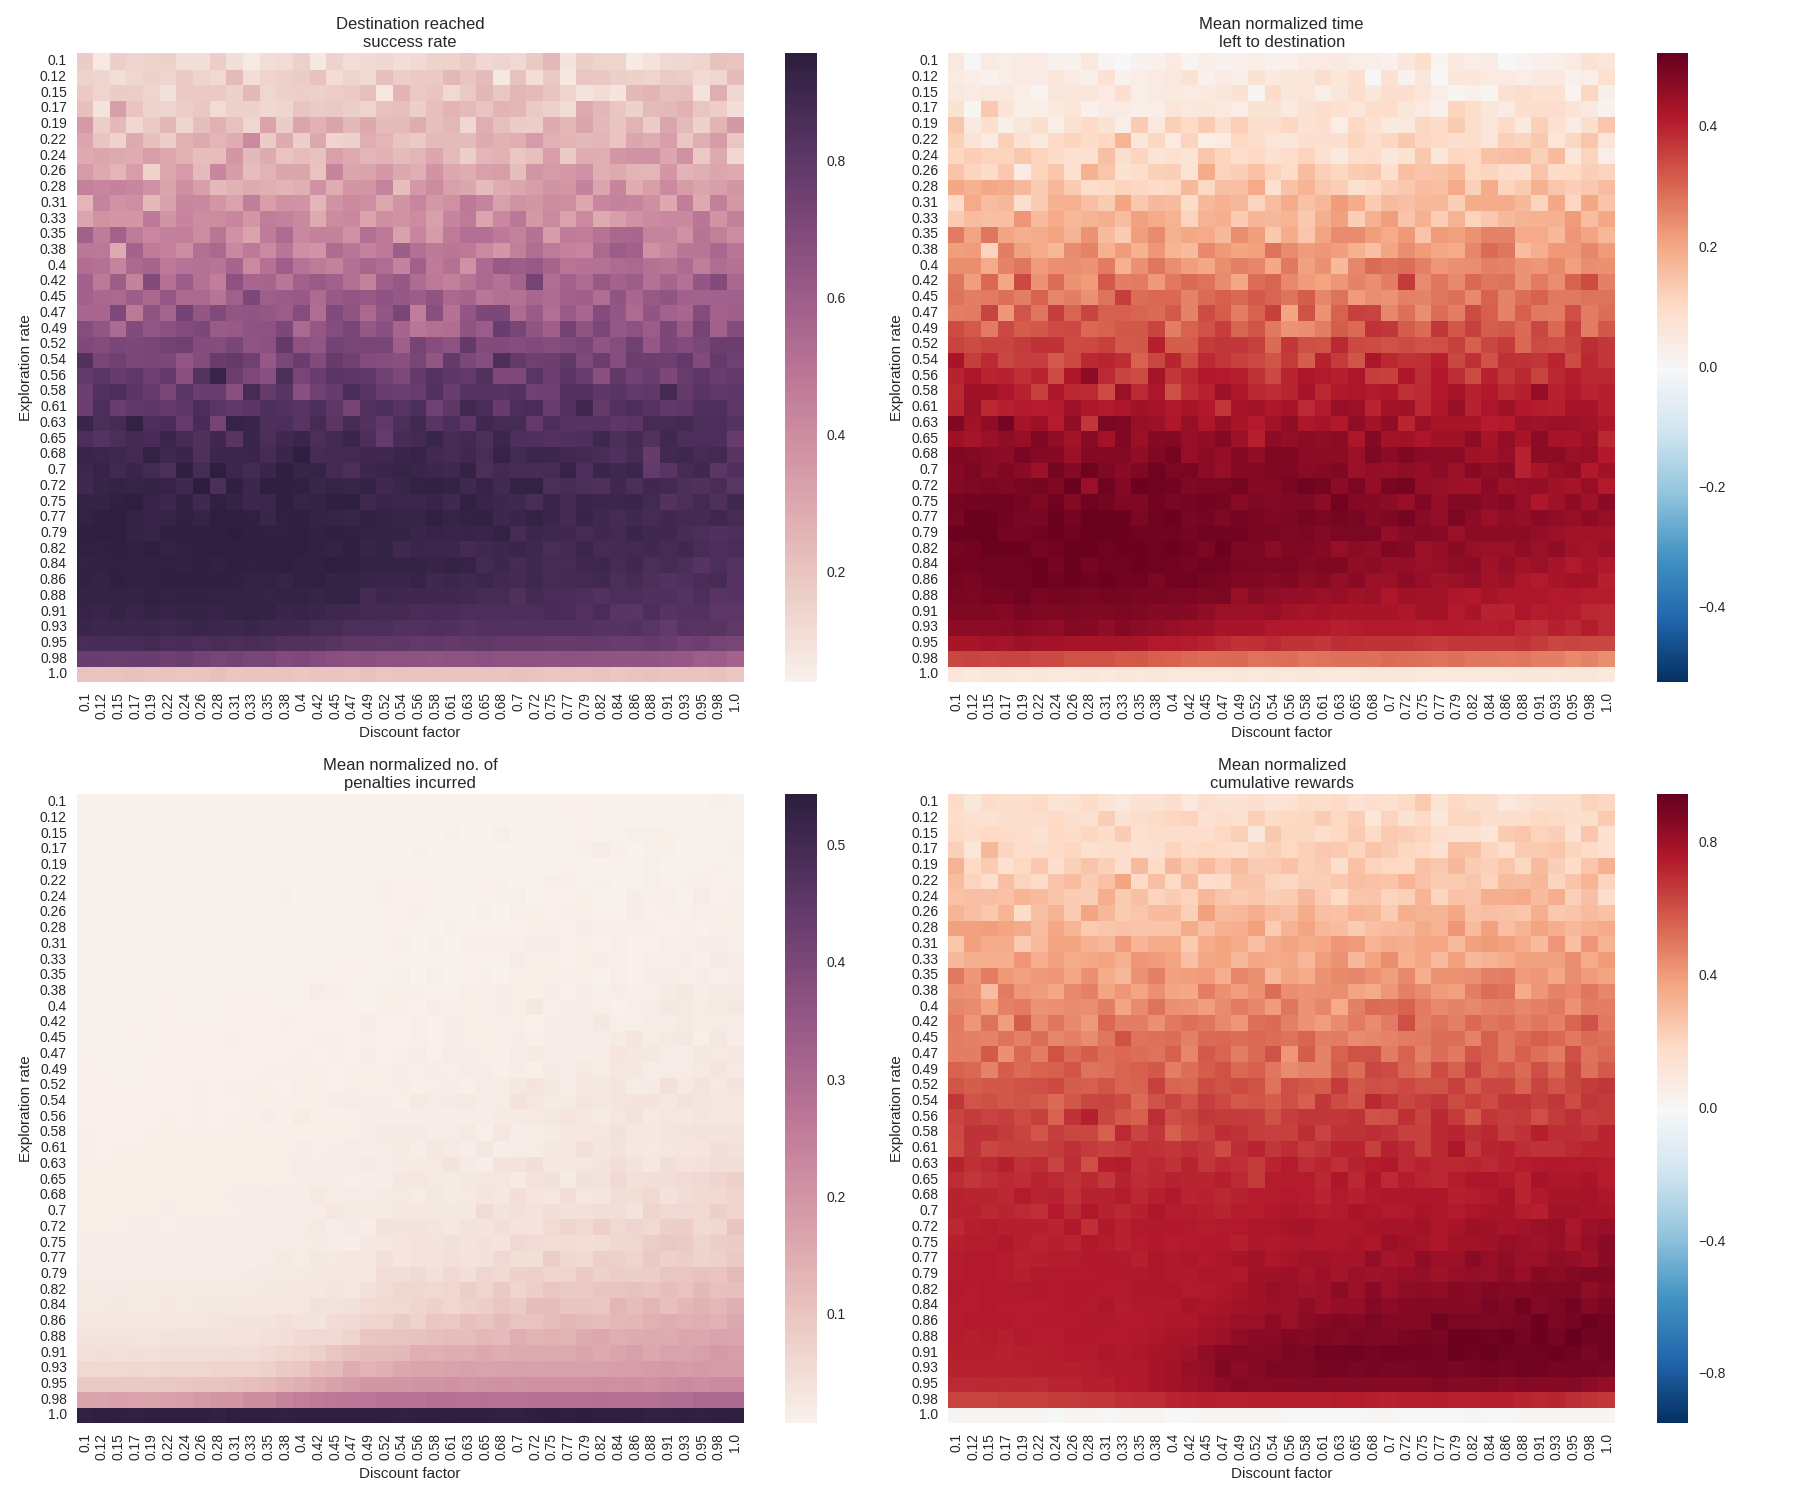
\includegraphics[scale=0.38]{plots_learning_1}
		\caption{Heatmaps of various measured observations with agent at learning factor ($\alpha\prime$) of $1.0$}
		\label{fig:learning_1}
	\end{figure}
	
	\begin{figure}[b]
		\centering
		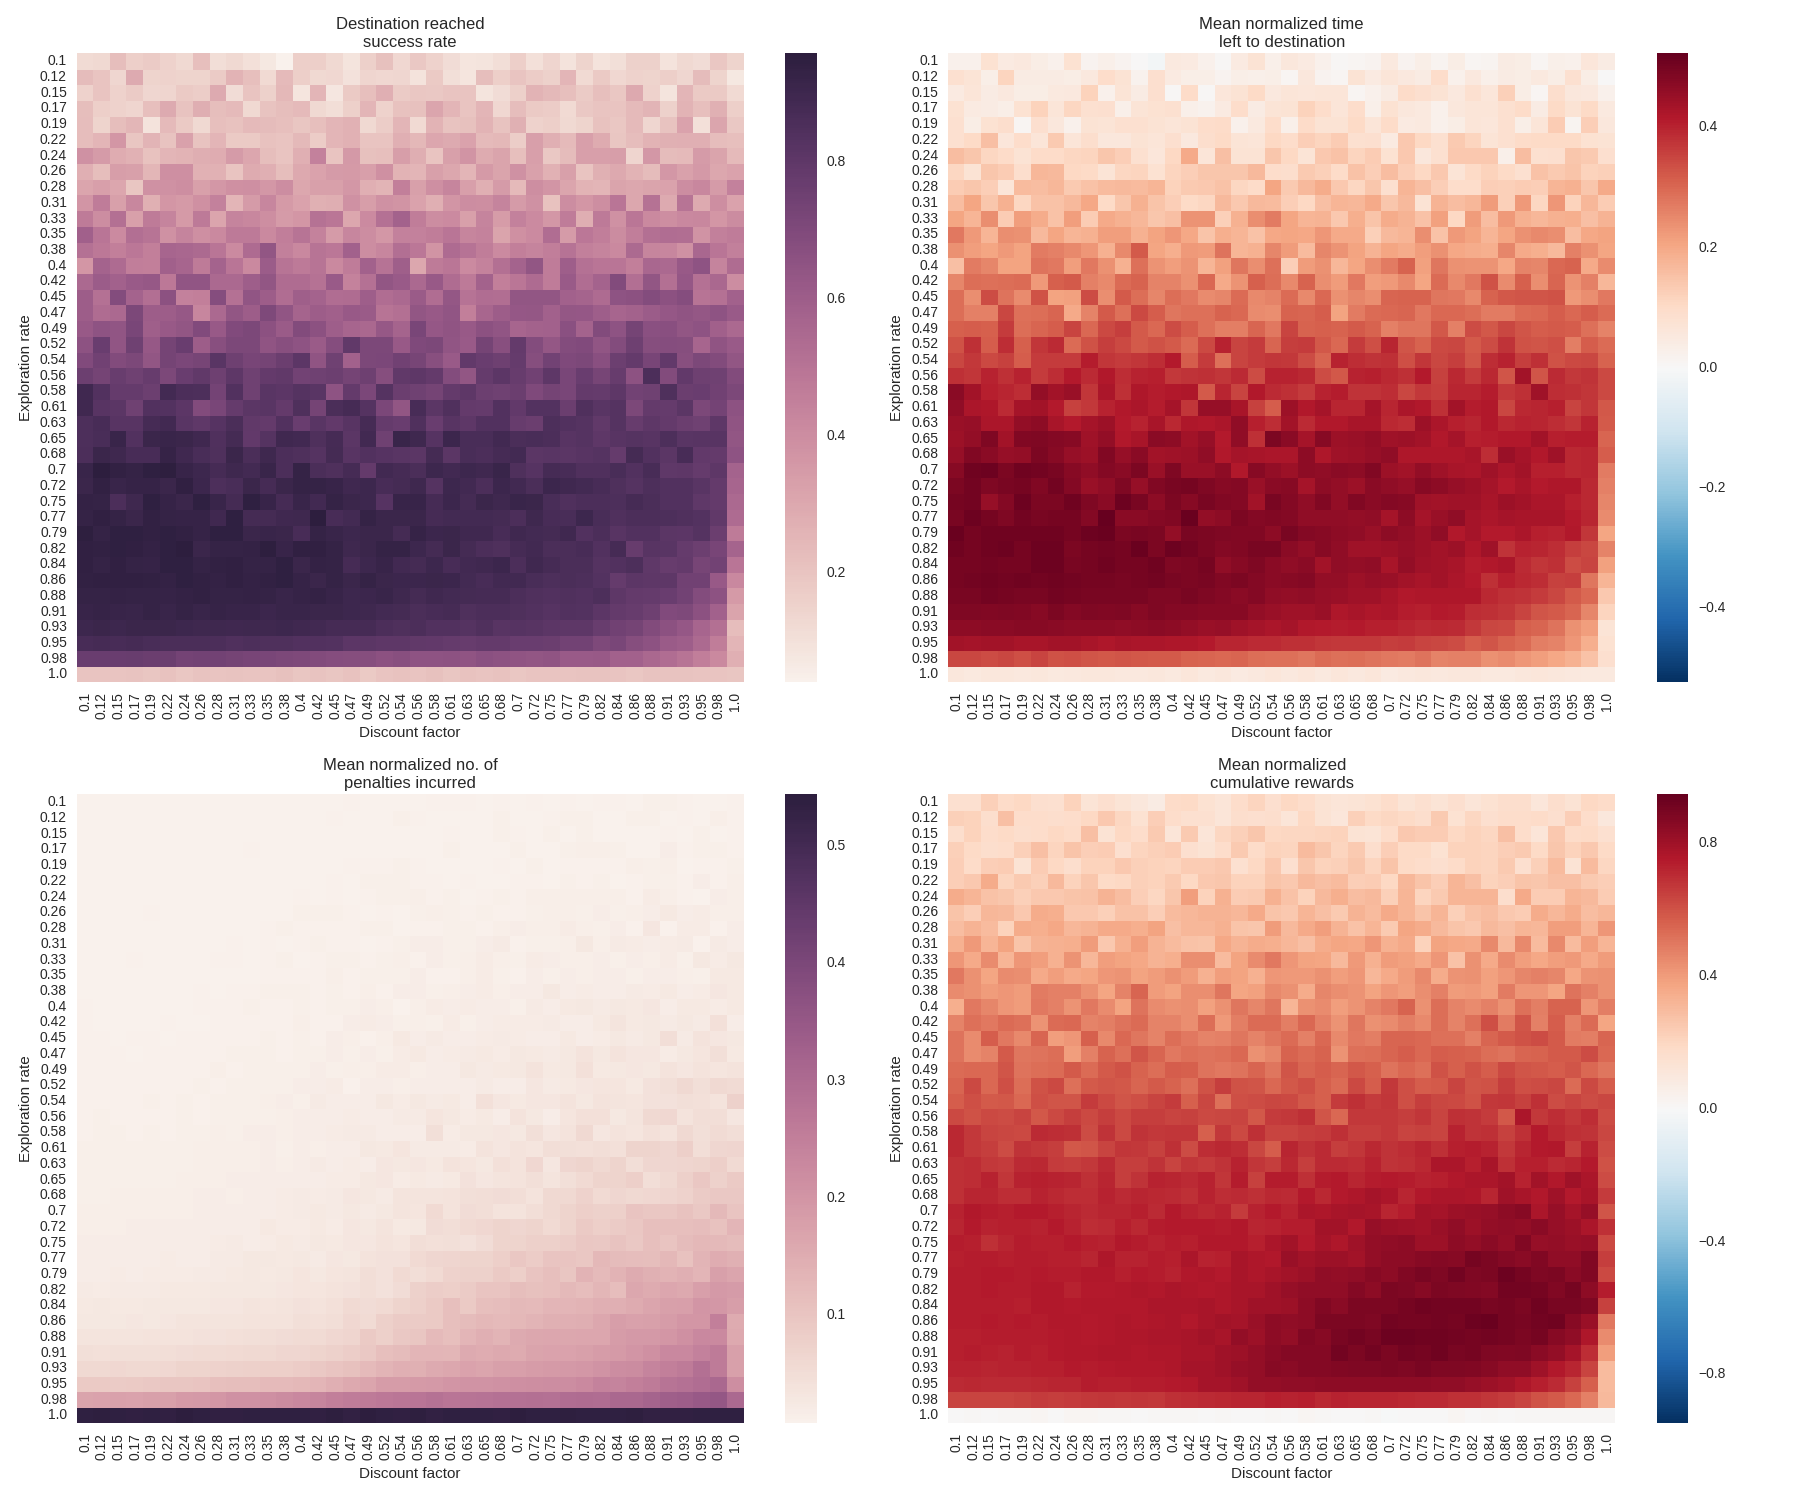
\includegraphics[scale=0.38]{plots_learning_4_5}
		\caption{Heatmaps of various measured observations with agent at learning factor ($\alpha\prime$) of $4.5$}
		\label{fig:learning_4_5}
	\end{figure}
	
	\begin{figure}[b]
		\centering
		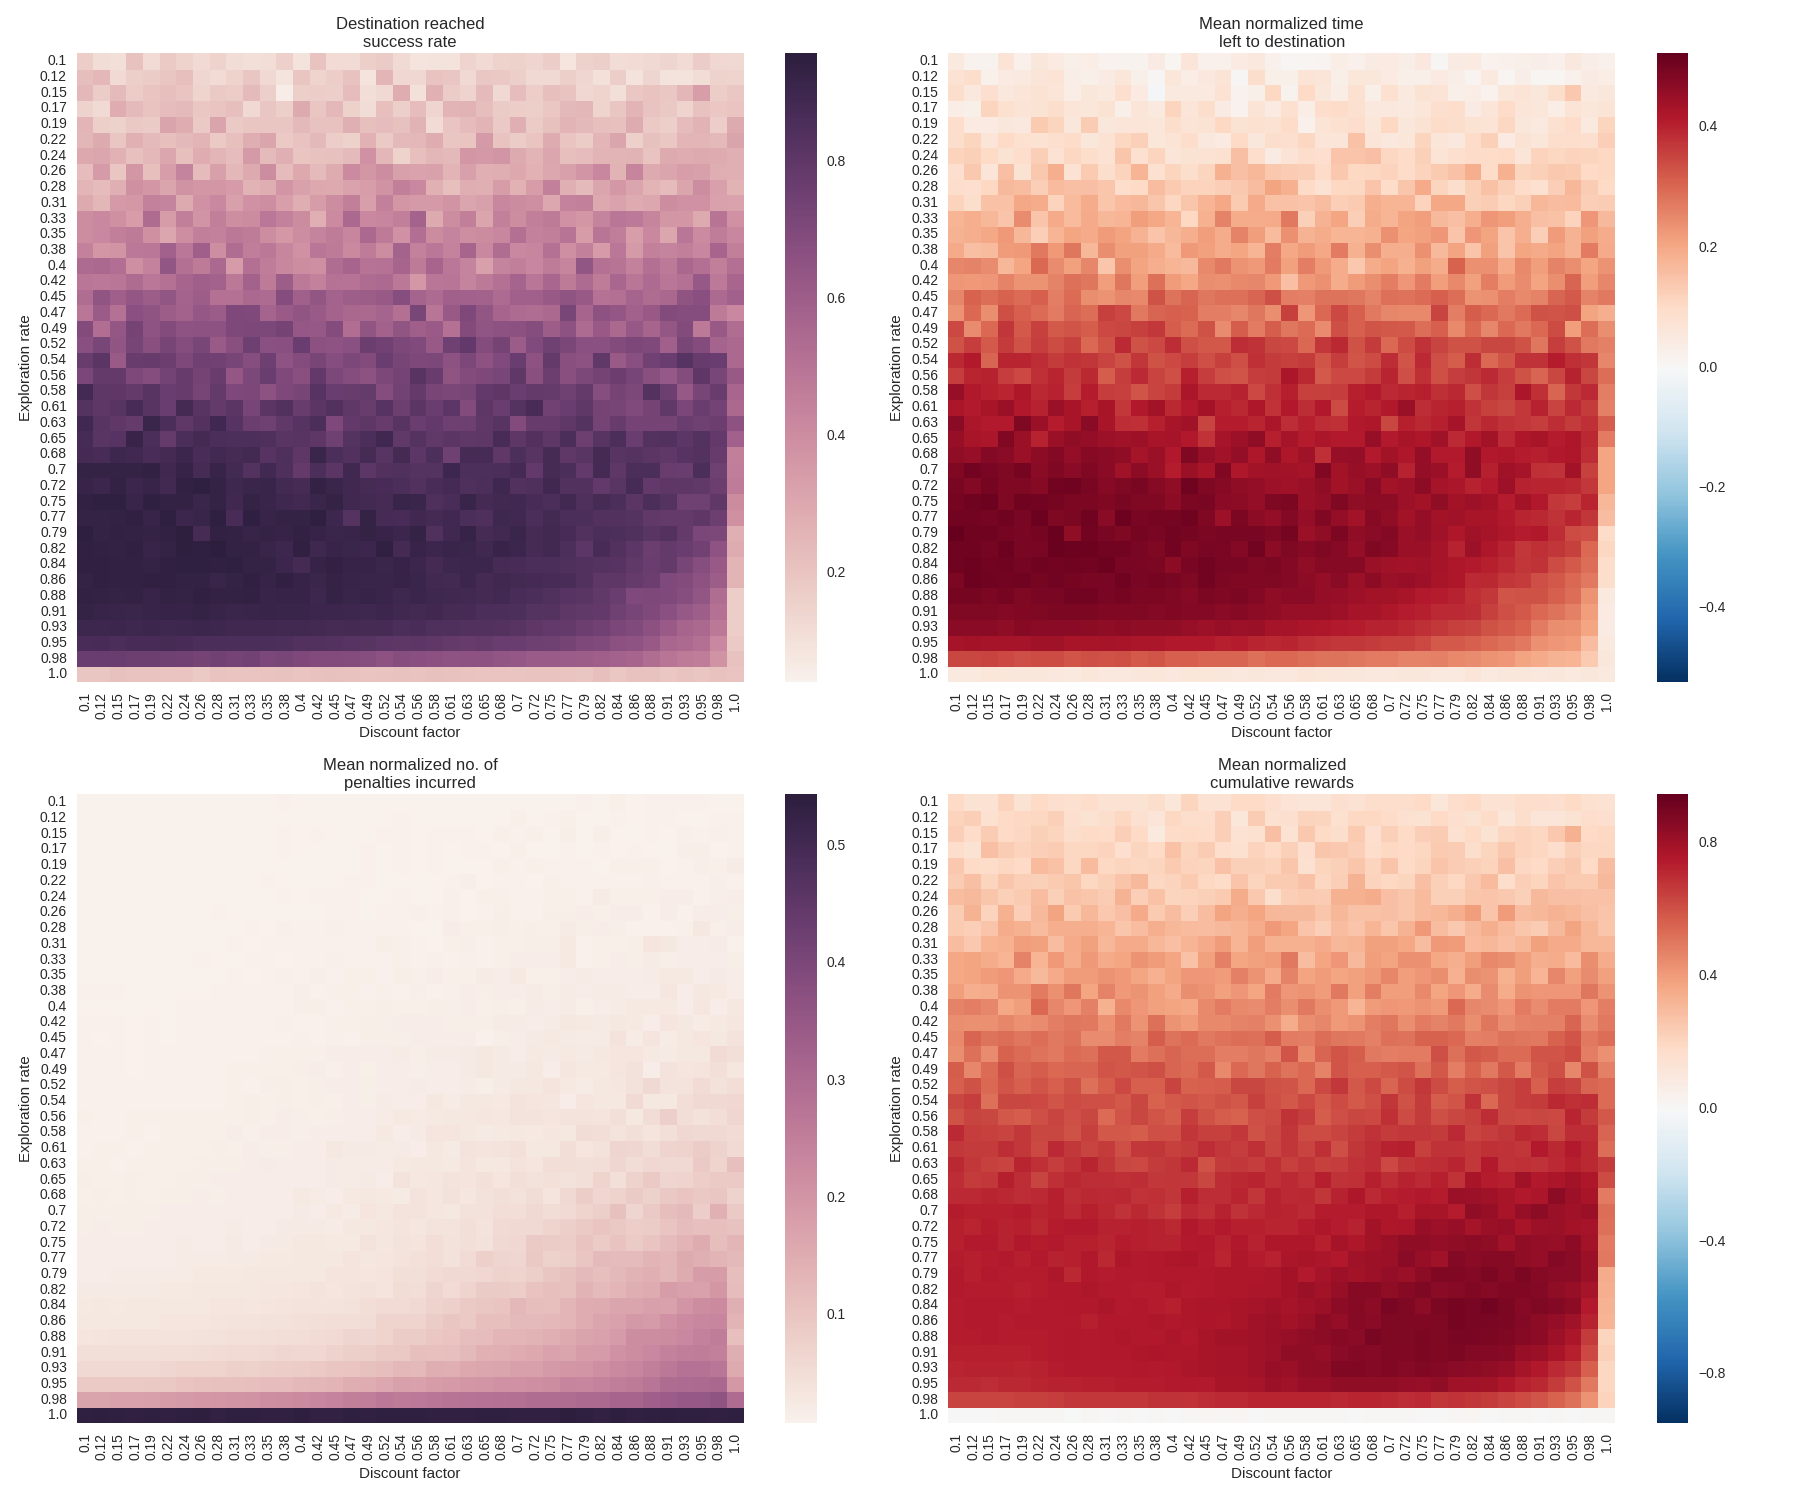
\includegraphics[scale=0.38]{plots_learning_8}
		\caption{Heatmaps of various measured observations with agent at learning factor ($\alpha\prime$) of $8.0$}
		\label{fig:learning_8}
	\end{figure}
		
	To assess the best parameters to the learning model, performance measurements were taken for a range of parameter values, viz., \emph{exploration\_rate} ($\epsilon$), \emph{discount\_factor} ($\gamma$) and \emph{learning\_factor} ($\alpha\prime$). For 3 different $\alpha\prime$, a parameter grid of size 40, spanning $[0.1,1]$ each was constructed for $\epsilon$ and $\gamma$. 40 simulations for each parameter set were performed, and for each trial in a simulation, results of the learner such as number of penalties incurred, cumulative rewards and time left after reaching destination were found out. These numbers were then normalized with the total time alloted by the planner for each trial. The mean of the normalized results and the destination reached success rate for each simulation (100 trials) are then computed and stored. The simulator script provided along with the project was slightly modified to accomplish this task. After running all the simulations (4800 in total), the stored results were plotted in heatmaps as shown in Figure \ref{fig:learning_1}, \ref{fig:learning_4_5} and \ref{fig:learning_8}. 
	
	A formal grid search is not performed to find the \emph{best} parameters, but the heatmaps aid (visually) to find the approximate optimal parameters. Following are some insights from the heatmaps, mainly considering Figure \ref{fig:learning_1} as a template:
	\begin{itemize}
		\item Heatmap corresponding to \emph{Destination reached success rate} relates to the likelihood of learning agent successfully reaching the destination within the dead line. It can be seen that with rising exploration factor, the success rate tends to increase. This is due to the fact that, the agent is able to discover the environment better and take actions accordingly. However, it is seen that with exploration criteria at 1.0, the success rate sharply dips again as agent never takes any learned actions. The discount factor has a rather shallow gradient, apart from in the extremes, where a slight dip is observed.
		\item The heatmap for \emph{Mean normalized time left to destination} correlates highly with the destination reached rate observations, with longer times left from deadline when agent reaches destination, for better combinations of exploration and discount factor.
		\item The heatmap for \emph{Mean normalized no. of penalties incurred} shows an interesting observation not as apparent in previously mentioned plots. As the discount factor increases, it can be seen that higher penalties are incurred at near optimal exploration rates. This is mainly because, with higher discount rates, the effect of Q-values of the neighbouring states (long term benefit) becomes higher, which makes the agent take certain penalties in hopes of a better long term reward. Also, it can be observed (rather uninterestingly) that with extreme exploration criteria, the agent incurs highest penalties.
		\item The effect of better long term rewards with higher discount factor can be observed even in the heatmap of \emph{Mean normalized cumulative rewards}, which represents the total reward an agent gets in a particular trial.
	\end{itemize}
	
	The observations corresponding to $\alpha\prime = 4.5$, and $\alpha\prime = 8.0$ follow similar trends to the $\alpha\prime = 1.0$. However, with higher $\alpha\prime$, the effect of higher discount rates (at extremes) become more apparent, and the overall observed positive trends become much less prominent (Ex: The highest destination reached success rate for $\alpha\prime = 8.0$ is lesser than that for $\alpha\prime = 1.0$).
	
	A formal parameter grid search was not performed because from the plots, it is apparent that the effectiveness of an agent can be context based. In other words, we see that lower discount factors favor higher destination reached success rates and time left at destination, as opposed to higher discount factors that favor higher cumulative rewards. Based on the desired incentives, which is subjective, the discount factor can be adjusted. Thus $\gamma = 0.4$ is chosen, that slightly favors better success rates. $\epsilon = 0.8$ is chosen as it appears to strike the \emph{sweet spot} in all the trends, and $\alpha\prime = 1.0$ is chosen as it gives the highest overall performance.
	
	With the above mentioned \emph{optimal} parameters, the agent achieves on average -- including the trials in which agent is in heavy exploration (for learning) -- success rate of $~95\%$, path completion time of about half that is allotted (dead line), and insignificant penalties. In any particular simulation, after about 5-10 trials, the agent starts to learn near optimal policy, and follows the planner almost always; the optimal policy for the situtation being the one in which the agent reaches the destination as fast as possible without breaking the rules of the road. For most simulations, the learned policy is near optimal because a particular deadlock situation (mentioned in Section \ref{notes}) that rarely occurs in trials, prevents the agent from reaching destination.
	
	\begin{figure}[b]
		\centering
		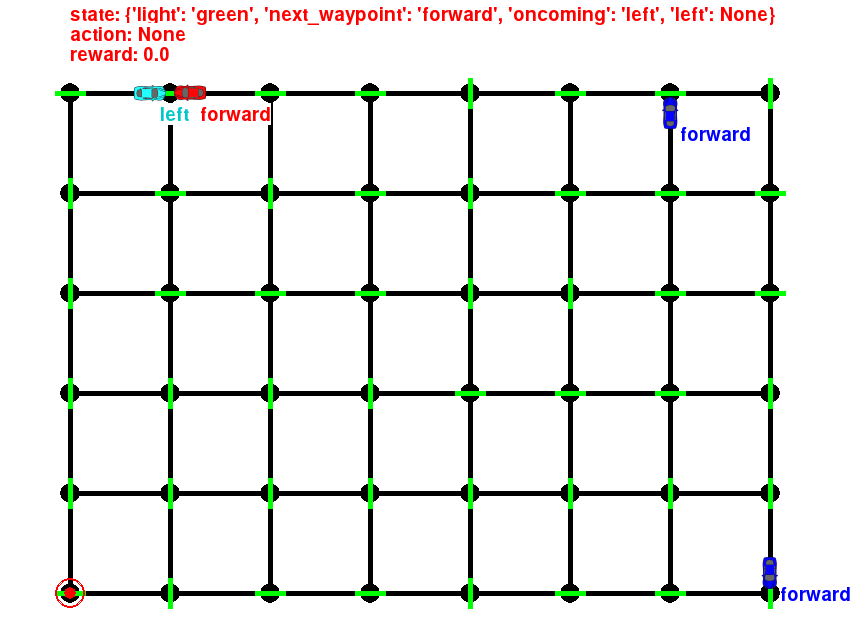
\includegraphics[scale=0.5]{conflict}
		\caption{Conflict of actions between learning agent and oncoming \emph{dummy} traffic, leading to a deadlock}
		\label{fig:agent_conflict}
	\end{figure}
	
	\section{Notes}	\label{notes}
	\begin{itemize}
		\item In many simulations with \emph{optimal} learning parameters, the learning agent sometimes gets \emph{stuck} at intersections. Figure \ref{fig:agent_conflict} shows the situation in which the learning agent (red car) remains forever at the intersection when oncoming traffic (blue car) wants to turn left. The learning agent learns to remain passive most of the times at this situation, although the rules of road give the agent the right of way. However, if enough such situations are encountered early during the learning -- which seldom is the case even with a exploration heavy parameter --, the agent learns to move forward at this juncture. So, it can be said that the agent learns near optimal policy most of the times, but in simulations when it learns to get out of this deadlock, the agent will have learnt the exact optimal policy.
		\item In the provided environment, it is hard to encode the deadline to motivate the learner in terms of time. If the rewards are made a function of time left to completion, this could probably be solved. However, this would make the system non-stationary, which is not ideal for Q-Learning. Another easy option could be to enforce a penalty for staying idle, which would go along well with Q-Learning. This alternative basically motivates the agent to \emph{stay on the move}. A preliminary experiment with the environment that rewards -0.5 for taking no action at an instant showed that the learner finishes the trials with sufficiently well success rate, albeit with less-than-ideal paths. This also helps avoid deadlocks mentioned previously.
		\item During implementation of the Q-Learner, it was found (by accident) that updating Q-values with a wrong combination of state transitions somehow gave equivalently \emph{well performing} learner. That is, if $s$ is state of agent obtained from \emph{sensing} the environment before taking action $a$ and $s\prime$ is the state after taking action with reward $r$, then the correct Q-Learning implementation uses the transition $<s, a, r, s\prime>$. The accidental input that inadvertently worked is $<s, a, r, s_{prev}>$ where $s_{prev}$ is the state of the agent \emph{sensed} before taking action in the previous iteration of \texttt{run()}. This aberration is likely due to some underlying symmtery in the reward/action scheme of the environment. For implementation, refer \href{https://github.com/QuaziRandom/MLND_Project_4/tree/870f14d912e8e9fbec4da7b2008cd2bf522f8b25}{commit}.
	\end{itemize}

\end{document}